
\section{Multiplanet retrieval}
\label{sec:exp_multis}

Finally, we turn from LCSim light curves to more realistic Lilith-4 light curves, which contain gaps and in some cases transit signals from multiple planets per light curve. The task in this experiment was to provide correct $t_0$ and $P$ for subset of transit signals in a subset of light curves of Lilith-4. 

The light curves that were used, were not used for training, validating or testing of the RNN as they were set aside for this experiment from the beginning. The first selection of light curves contained all light curves that had more than one sector of data available. Subsequently, all light curves with EBs or BEBs were filtered out, as well as light curves that contained no transit signals. Counting each sector individually, we are then left with 6511 light curves. Only a subset of the transit signals is used for evaluation. For example, we ignored all transit signals that occurred less than three times in a single light curve, or had a period smaller than two days. For these choices, 3841 of the light curves contained no transit signals that were used for evaluation, 2130 contained transit signals of a single planet, 474 of two different planets, 57 of three different planets and 9 of four different planets.

One baseline in this experiment is BLS-12h from Section \ref{sec:exp_singles}. Another baseline is the TESS pipeline, for which the detections for this data set are publicly available\footnote{\url{https://archive.stsci.edu/missions-and-data/tess/data-products/lilith-4}}. However, as opposed to BLS, we have no control over the amount of candidates that are returned by the pipeline. In fact, the pipeline has already set a detection threshold, so we cannot anymore evaluate the entire range of thresholds to analyze the trade-off between precision and recall. \todo{explain light curve preprocessing for BLS (outlier removal, detrending)}.

We only used PTS-Fold for this experiment, because it was most competitive to BLS in the previous experiment. The gaps in the low-risk detrended light curves were filled by linear interpolation, and centroid data was used as additional input to the RNN that is used as the basis of PTS-Fold. Again, both PTS-Fold and BLS-12h were allowed to return a maximum of three candidate detections, even though there are a few samples with four separate transit signals. This was mainly to reduce the computation time for BLS.

Figure \ref{fig:multis-pr} shows the precision-recall curves for each detection method in the given task. Again, the curves differ strongly from the ones in figures \ref{fig:monos-pr} and \ref{fig:singles-pr}. For the pipeline detections, this is because we only have detections above the pre-selected threshold available. The results shown here were obtained by setting different thresholds on the SNR provided with each pipeline detection, to define new sets of detections for each threshold. For PTS-Fold and BLS-12h, it is notable that both approach a recall of 1, for gradually decreasing precision. The reason for this behaviour is not entirely clear \todo{edit text according to new figure. there was a bug which is now fixed and the figure is updated}. Another interesting point is that there is no clear winner between PTS-Fold and BLS-12h in this experiment. Although PTS-Fold has the highest precision for low values of recall, BLS-12h seems to be in favor for larger recall values. In addition, the area under the curve (AUC) for both methods indicate that BLS-12h had a slightly higher average precision over the full range of recall values.
\todo{write a bit more, also mention how many planets were found by one method which were not found by the other}

\begin{figure}
    \centering
    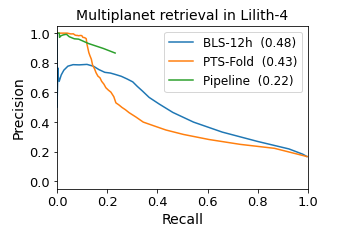
\includegraphics[width=0.4\linewidth]{Experiments/Figures/Multis/multis_pr.png}
    \caption{\todo{caption; between brackets shows area under the curve (AUC), also interpreted as average precision} \todo{explain that we have no uncertainties, and these results therefore only tell something about this specific experiment. future research should confirm these findings.}}
    \label{fig:multis-pr}
\end{figure}